\documentclass{bioinfo}
\copyrightyear{2014}
\pubyear{2014}




%%% Additional Macro and command.
\usepackage{url}
\newcommand{\pkg}[1]{{\fontseries{b}\selectfont #1}}
\makeatletter
\newcommand\code{\bgroup\@makeother\_\@makeother\~\@makeother\$\@codex}
\def\@codex#1{{\normalfont\ttfamily\hyphenchar\font=-1 #1}\egroup}
\makeatother
\let\proglang=\textsf
%%% End of additional Macro and command.


\newcommand{\package}{ribModel}


%%% Start here.
\begin{document}
\firstpage{1}

\title[ribModel]{ribModel: an \proglang{R} package for codon usage bias fits}
\author[
Landerer \textit{et~al}]{Cedric Landerer\,$^{1,3}$\footnote{
to whom correspondence should be addressed
},
Alex Cope\,$^{1,4}$
Russell Zaretzki\,$^{2,3}$, and
Michael Gilchrist\,$^{1,3}$
}
\address{$^{1}$
Department of Ecology and Evolutionary Biology,
$^{2}$Department of Statistics, Operations, and Management Science, and
$^{3}$National Institute for Mathematical and Biological Synthesis,
University of Tennessee, Knoxville, TN, USA,
$^{4}$Oak Ridge National Labratory, Oak Ridge, TN, USA} 
\history{Received on XXXXX; revised on XXXXX; accepted on XXXXX}

\editor{Associate Editor: XXXXXXX}

\maketitle

\begin{abstract}

\section{Summary:}
\pkg{\package} is a collection of codon models, estimating terms related to mutation and selection coefficients of synonymous codon usage bias (CUB) and population genetics parameter of interest. 
The implemented models allow to analyze sequence data as well as ribosome foot printing data to estimate selection on ribosome overhead cost, nonsense error rate and ribosome pausing times. 
\package also allows for the estimation of the evolutionary average protein synthesis rate, reflecting the environmental conditions an organisms evolves under. 
\package implements a Metropolis-Hastings withing Gibbs sampling to fit the codon models.
The framework provides an R interface for ease of use and is implemented with a generic design to allow for future additions of additional codon models.

\section{Availability:}
\pkg{\package} and documents are freely available under the Mozilla Public License 2.0
on CRAN (\url{http://cran.r-project.org/package=cubfits}).

\section{Contact:} \href{cedric.landerer@gmail.com}{cedric.landerer@gmail.com}
\end{abstract}


\section*{Introduction}

\begin{itemize}
\item Huge influx of genome scale data sets across the tree of life
\item Why study CUB?
	\begin{itemize}
	\item CUB is shaped by mutation and selection
	\item informs about selection on translation efficiency.
	\item translation efficiency can mean ribosome pausing, error free translation (nonsense or missense errors).
	\item CUB potentially relates to co-translational folding. Tools allows to get at questions
	\end{itemize}
\item compare to CAI and tAI
	\begin{itemize}
	\item CAI and such require reference set of house-keeping gens for comparison of adaptation
	\item tAI uses tRNA copy number implying no other factors are involved
	\item We have population genetics component getting at $N_e * s$ with our model
	\end{itemize}
\item inference of expression as evolutionary mean unaffected by growth conditions and experimental noise
\item Bayesian MCMC method allows for priors and multilevel and hierarchy 
\end{itemize}



\section*{Results}
\begin{itemize}
\item Performance (simulated data)
	\begin{itemize}
	\item runtime by number of genes and number of mixtures
	\item confidence in parameters by number of genes
	\item estimation of phi values (gene ordering)
	\end{itemize}
\item $s_{epsilon}$ as a measure of noise due to the lab conditions by eliminating technical 			noise. Use replicates to estimates technical noise

\item 
\end{itemize}


\section*{Introduction}
Driven by improvements in DNA sequencing technology and methodology, the past 15 years has seen an exponential growth in the number of publicly available genomes. 
This influx of genomic data necessitated the development of computational tools which allow researchers to extract information.

Information about selection on the translation process, such as factors shaping translational efficiency and co-translational folding, can be extracted using codon usage bias.
CUB refers to non-uniform usage of synonymous codons shaped by bias in mutation and selection.
Although CUB was first studied almost 40 years ago, many questions related to the factors shaping CUB remain open.
As a result, many metrics were developed in an attempt to quantify CUB, such as Codon Adaptation Index (CAI).
There are many issues with these metrics.
For example, CAI relies on a reference set of genes assumed to be highly expressed, such as genes coding for ribosomal proteins.
Most of these metrics only account for selection in shaping CUB and is not rooted in population genetics. 
Recent work demonstrated that to accurately quantify CUB, mutation bias and genetic drift are also needed.
In [Gilchrist et al 2015], a mechanistic model rooted in population genetics that accounted for selection, mutation bias, and genetic drift was presented. 
Here, we describe an open-source computational tool that allows researchers to analyze CUB data using the model presented in [Gilchrist et al 2015].
In addition this work expands Gilchrist et al 2015 by allowing for mixture distributions for mutation and selection within a dataset.

Information on mutational and selection processes can be obtained from codon usage bias.
 
The influence of mutation and selection is related to the evolutionary averge protein production rate $\phi$ of a gene.
Genes with increased protein synthesis rate are belived to be under higher selection for translation efficiency and are therefore composed of a higher percentage of optimal codon.
Gene regions that deviate from that pattern can indicate to explore differential selection on codon usage for the purpose of co-translational folding or signal peptides


\begin{figure*}[!tpb]
\centering
 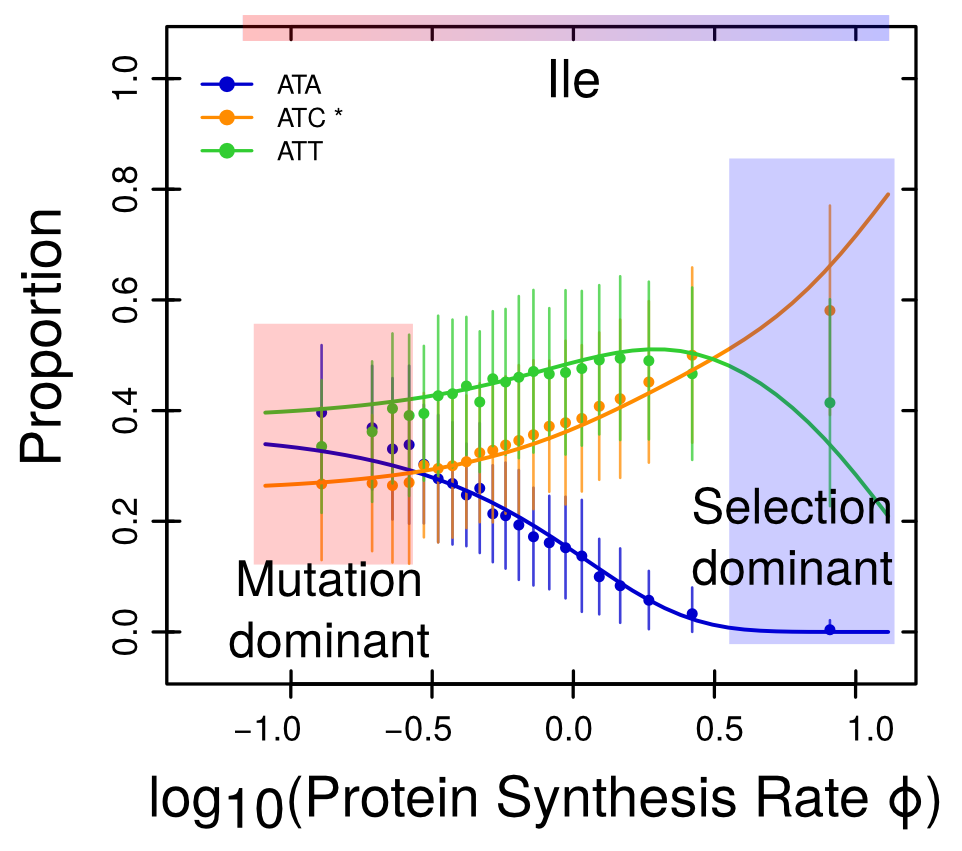
\includegraphics[width=3.5in]{expl_model.png}
\vspace{-0.2cm}
\caption{Binning for amino acid Isoleucin by expression levels (y-axis) where dots are mean proportions of synonymous codons (x-axis) of 100 simulated sequences in every 5\% expression windows, and vertical lines are 90\% empirical intervals. The curves are theoretical prediction of codon usages.
}
\label{fig:plotbin}
\end{figure*}

\section{Features}
\subsection{Code structure}
ribModel follows the classical design principles of object orientation and inheritance (Booch 1993). 
The software package consists of two partially virtual base classes (Model, Parameter) which hold basic functionality shared between all models and guarantee that required functionality is available in each child class (e.g. ROCModel).
The core of the package is the class MCMC which provides a member function run. 
run requires as input a model and a genomic dataset represented by the classes Model and Genome. 
The inheritance structure makes it unnecessary for the run function to require information about the type of model it analyzes.
The class MCMC implements a conditional Markov Chain Monte Carlo structure (Metropolis-Hastings within Gibbs sampling) where model parameter can be separated into three categories, codon/amino acid specific; gene specific; or hyper parameters. 
This assumed structure does not require that all models have to contains all three types of parameters, but merely allows to split parameters into these type for more efficient sampling.
\subsubsection{Writing extensions}
The framework was designed to allow for simple extensions, providing new models to analyze genomic data. 
While the usage of the package does not require any knowledge of C++, extending the framework with new models requires C++ expertise. 
For a new model to be included, a new child class of Model and Parameter has to be defined.
The child class inherits all necessary functionality and function definitions from the base class. This ensures compatibility of the newly defined model with the evaluation environment.
Thus only the implementation of the likelihood function is required. 
However, child classes are allowed to modify or override existing functionality inherited from the base class. 
It is however required that the function definition is consistent with the base class. 
Base classes can also be extended by their child classes, adding additional functionality the base class does not provide.
\subsubsection{Merging R and C++}
R provides native support for the integration of C and FORTRAN. 
However, R does not provide a native C++ support, which is necessary to implement an object oriented software design. 
To allow for the implementation in C++, I utilized the R package Rcpp (Eddelbuettel \& Francois 2011). 
Rcpp provides a module structure allowing the exposure of whole C++ classes to R. 
R represents each instance of a class (Object) as a pointer to an environment. 
Unlike with a regular R environments, interaction with an object is limited to the functionality of the class the object is an instance of.
While R users are mostly familiar with classes that allow for the modifications of their internal structure (S3 class), a class exposed with Rcpp, like S4 classes, are self-contained and the internal structure of an object always rejects the class definition. 
This prohibits users from accidentally or purposefully changing objects such that they do no longer match their class definition.
In R, the change to self-consistent objects comes with a change of syntax, unfamiliar to most R users. 
To avoid any complications, S3 style R wrapper functions are provided to ease the use of the package and avoid confusion.

\section*{Discussion}
\begin{itemize}
\item Runtime, scalability
\item Extendability, FONSE, PANSE, RFP
\item applications, hybridization, phylogenetics, variation in mutation and selection
\end{itemize}



%\bibliographystyle{natbib}
%\bibliography{bioinfo}
\end{document}